\section{Specifiche del prodotto}
	I contenuti della specifica saranno presentati seguendo l'approccio top-down: dalla descrizione macroscopica del sistema si scenderà sempre più in dettaglio passando alla descrizione delle singole componenti. Verranno inoltre descritti i design pattern utilizzati e come essi sono stati applicati. Per agevolare la comprensione si è scelto di utilizzare i diagrammi dei package, delle classi, di attività e di sequenza, descritti attraverso lo standard UML 2.0.
	
	\subsection{Architettura generale del sistema}
	Il sistema Quizzipedia è di tipo \emph{client-server}; il \emph{client} fornisce all'utente un'interfaccia web su browser per la creazione e fruizione di questionari, mentre il lato \emph{server} si occupa di gestire e salvare i dati su DBMS PostgreSQL. La base di dati raccoglie principalmente quesiti memorizzati in QML, che su richiesta verranno elaborati da un interprete.
Il suddetto interprete processa l'input QML, precedentemente validato nella forma da un parser apposito, traducendolo in linguaggio HTML5 visualizzabile da browser.
Nella realizzazione del sistema Quizzipedia verrà adottato il design pattern \emph{Model View Presenter} nella sua variante \emph{Passive View}.
\begin{figure}[h!]
\begin{center}
	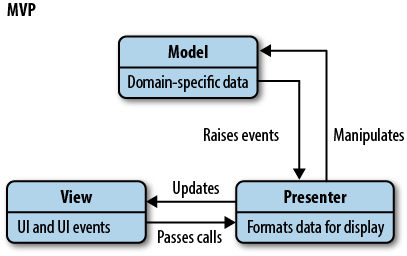
\includegraphics[scale=1.3]{../images/mvp.png}
	\caption{Il design pattern Model View Presenter (Passive View)}
\end{center}
\end{figure}
\begin {itemize}
\item\textbf{Model}: definisce l'organizzazione dei dati e ne specifica le modalità di accesso. Nel sistema Quizzipedia è situato nella parte server che opera sulla sottostante base di dati. Fa parte del Model anche la componente \emph{Parser} che opera sui dati prima che essi vengano salvati nel DBMS.
\item\textbf{View (Passive)}: rappresenta l'interfaccia grafica presentata all'utilizzatore, la quale visualizza i dati e cattura le interazioni dell'utente. L'aggettivo "Passive" indica che la View non è responsabile del proprio aggiornamento al variare del Model, compito che ricade sul Presenter.
\item\textbf{Presenter}: controlla la View e ne gestisce il comportamento in reazione alle interazioni dell'utente, interagisce di conseguenza col Model per ottenere i dati necessari.
Una volta ottenuti i dati si preoccupa di aggiornare la View. Nel sistema Quizzipedia implementa la parte logica, affiancata a quella grafica, del Client. Realizza un totale disaccoppiamento tra Model e View, controllandone i flussi di comunicazione.
	\end {itemize}
	Altre possibili architetture che sono state prese in considerazione sono definite dai design pattern \emph{Model View Controller (MVC)} con \emph{Front Controller}, \emph{Model View Presenter (MVP)} nelle varianti \emph{Presentation Model} e \emph{Supervising Controller}, e il design pattern \emph{Model View ViewModel (MVVM)}.
	\begin{itemize}
	\item La prima pone il Controller, componente simile al Presenter, nella parte server del sistema. Quest'opzione è stata scartata per evitare di aumentare troppo la complessità del lato server, ponendo invece il Presenter dal lato client, così da redistribuire responsabilità e carico di lavoro.
	\item Il \emph{Presentation Model} invece è affine al design pattern scelto, ma impone che sia la componente View ad aggiornarsi autonomamente al variare del Model. Proprio per questo motivo si è deciso di scartarla in favore del Passive View: per disaccoppiare completamente le componenti Model e View, e per alleggerire ulteriormente quest'ultima concentrandone tutta la parte logica nel Presenter.
	\item Il \emph{Supervising Controller} propone che la View si aggiorni autonomamente nel caso di piccole modifiche (tramite data-binding col Model), lasciando le manipolazioni più complicate al Presenter; è stato scartato in favore del disaccoppiamento totale tra View e Model.
	\item Il pattern \emph{MVVM} prevede di creare per ogni View un ViewModel, che rappresenta tutte le informazioni e i comportamenti della corrispondente View. La View si limita infatti, a visualizzare graficamente quanto esposto dal ViewModel, a riflettere in esso i suoi cambi di stato oppure ad attivarne dei comportamenti (tramite data-binding). Tale architettura è indicata per applicazioni particolarmente dinamiche in cui View e Model devono essere costantemente aggiornati. Non è questo il caso di Quizzipedia.
	\end{itemize}
	\subsection{Descrizione del componente Model}
	Il Model, situato nella parte server del sistema svolge le seguenti funzioni:
	\begin{itemize}
		\item Interagisce con un database PostgreSQL nel quale vengono salvati i dati del sistema (ad es. domande, statistiche, utenti). Fornisce quindi adeguate funzionalità di salvataggio e caricamento da database di tali dati.
		\item Al momento del salvataggio di una nuova domanda esegue il \emph{parsing} del codice QML tramite un componente chiamato \emph{Parser}. Se la domanda è sintatticamente corretta può essere salvata nel database.
		\item Offre un'interfaccia logica di accesso al Presenter attraverso la quale richiedere dati e operazioni su di essi.
	\end{itemize}
	\subsection{Descrizione del componente View}
	La componente View rappresenta l'interfaccia grafica che visualizza i dati del Model e inoltra i comandi dell'utente (o gli eventi da esso generati) al Presenter che si occuperà di gestire tali richieste sui dati interagendo col Model; la View si occupa quindi solamente della rappresentazione grafica dei dati e non ha alcun contatto diretto con essi. Essendo un'interfaccia web verrà realizzata tramite HTML5 e CSS3 per le parti statiche e con l'utilizzo di Javascript per le parti dinamiche. Per assicurare uno stile coerente tra le pagine web e migliorare l'adattabilità a piattaforme mobile verrà utilizzato il framework \emph{Materialize}.
	\subsection{Descrizione del componente Presenter}
	Il Presenter ricopre tre ruoli fondamentali: recepire ed elaborare gli input dell'utente,
comunicare col Model, ed aggiornare il View con i dati ottenuti. Per poterlo fare possiede le seguenti caratteristiche:
	\begin{itemize}
		\item Conosce i riferimenti alle altre due componenti. Il Presenter è l'unica componente che conosce entrambe le altre e facendo da singolo tramite tra Model e View permette il loro totale disaccoppiamento;
		\item E' in grado di elaborare gli input della View e tradurli in azioni sul Model. Viceversa ad ogni modifica del Model si preoccupa di aggiornare di conseguenza la View.  
		\item E' responsabile della traduzione delle domande dal formato QML a formato HTML visualizzabile da browser, tramite un componente \emph{Interpreter}.  Tale funzionalità viene richiesta ogni qualvolta il Presenter richiede e riceve dal Model una domanda in formato QML.
		\item Possiede dei gestori che possano modificare l'aspetto della View in reazione all'interazione dell'utente o ai dati ricevuti dal Model. Al suo interno il Presenter contiene delle classi che in risposta ad un evento, quale l'interazione dell'utente con la View o il ricevimento di una risposta dal Model, modificano l'aspetto della GUI presentata.
		\item Gestisce la somministrazione di un questionario ad un utente, domanda dopo domanda, fino alla consegna e valutazione.
	\end{itemize}
	\newpage